\documentclass{standalone}
\usepackage{tikz}

\begin{document}
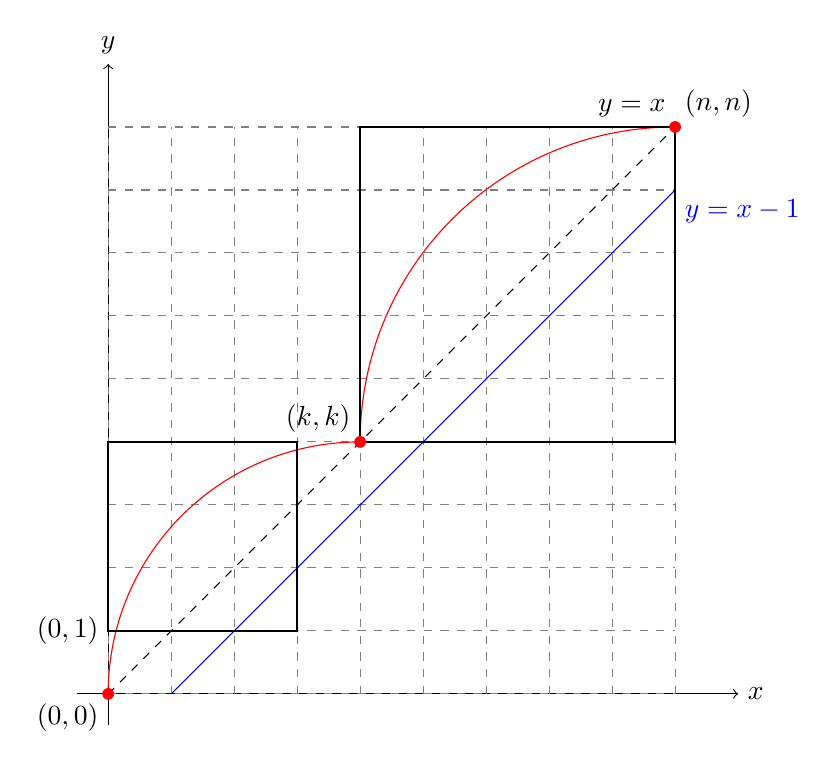
\begin{tikzpicture}[scale=0.8]
  % Axes
  \draw[->] (-0.5,0) -- (10,0) node[right] {$x$};
  \draw[->] (0,-0.5) -- (0,10) node[above] {$y$};
  
  % Grid lines
  \foreach \x in {0,1,...,9}
    \draw[dashed, gray] (\x cm,0) -- (\x cm,9);
  \foreach \y in {0,1,...,9}
    \draw[dashed, gray] (0,\y cm) -- (9,\y cm);
    
  % Line y=x
  \draw[dashed, black] (0,0) -- (9,9) node[above left] {$y=x$};
  % Line y=x-1
  \draw[blue] (1,0) -- (9,8) node[below right] {$y=x-1$};
  
  
  
  % Red arc from (0,0) to (2,2)
  \draw[red] (0,0) to[out=90,in=180] (4,4);
  \draw[red] (4,4) to[out=90,in=180] (9,9);
  
  % Fluorescent green square from (0,0) to (3,3)
  \draw[black!80!black, thick] (0,1) rectangle (3,4);
  \draw[black!80!black, thick] (4,4) rectangle (9,9);

  % Red point at (2,2)
  \node[circle, fill=red, inner sep=1.5pt] at (0,0) {};
  \node[circle, fill=red, inner sep=1.5pt] at (4,4) {};
  \node[circle, fill=red, inner sep=1.5pt] at (9,9) {};
    
  % Labels
  \node[below left] at (0,0) {$(0,0)$};
  \node[left] at (0,1) {$(0,1)$};
  \node[above left] at (4,4) {$(k,k)$};
  \node[above right] at (9,9) {$(n,n)$};
\end{tikzpicture}
\end{document}
